\documentclass[10pt]{article}
\usepackage{mathtools}
\usepackage{amsfonts}
\usepackage{pifont}
\usepackage{tkz-graph}
\usetikzlibrary{graphs}
\author{BM Corser}
\title{Discrete Assignment 3}
\begin{document}
    \maketitle 
    \begin{enumerate}
        \item 
        \begin{enumerate}
            \item Two non-isomorphic graphs with degree sequence $[2,2,2,2,3,3,4]$ are
                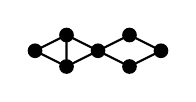
\begin{tikzpicture}[scale=0.4, every node/.style={scale=0.4}]
                    \SetVertexNoLabel
                    \GraphInit[vstyle=Classic]
                    \Vertex[x=0, y=0]{1}
                    \Vertex[x=1, y=-0.5]{2}
                    \Vertex[x=1, y=0.5]{3}
                    \Vertex[x=2, y=0]{4}
                    \Vertex[x=3, y=-0.5]{5}
                    \Vertex[x=3, y=0.5]{6}
                    \Vertex[x=4, y=0]{7}

                    \Edge(1)(2)
                    \Edge(1)(3)

                    \Edge(2)(3)

                    \Edge(2)(4)
                    \Edge(3)(4)

                    \Edge(4)(5)
                    \Edge(4)(6)

                    \Edge(5)(7)
                    \Edge(6)(7)
                \end{tikzpicture} and
                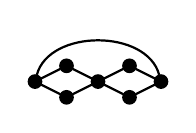
\begin{tikzpicture}[scale=0.4, every node/.style={scale=0.4}]
                    \SetVertexNoLabel
                    \GraphInit[vstyle=Classic]
                    \Vertex[x=0, y=0]{1}
                    \Vertex[x=1, y=-0.5]{2}
                    \Vertex[x=1, y=0.5]{3}
                    \Vertex[x=2, y=0]{4}
                    \Vertex[x=3, y=-0.5]{5}
                    \Vertex[x=3, y=0.5]{6}
                    \Vertex[x=4, y=0]{7}

                    \Edge(1)(2)
                    \Edge(1)(3)

                    \Edge[style={bend left=75}](1)(7)

                    \Edge(2)(4)
                    \Edge(3)(4)

                    \Edge(4)(5)
                    \Edge(4)(6)

                    \Edge(5)(7)
                    \Edge(6)(7)
                \end{tikzpicture}.
            \item 
                The graph $G$ is simple because it has no loops (no non-zero
                entries on the main diagonal of its adjacency matrix) and all
                other entries are either 0 or 1. By the handshaking lemma, the
                number of edges in a simple graph is equal to half the sum of
                the degrees of its vertices. The sum of entries of a row in an
                adjacency matrix is the degree of the corresponding vertex. As
                such, half of the sum of all entries in an adjacency matrix of
                a simple graph gives the number of edges of that graph. Here,

                $\frac{0 + 0 + 1 + 1 + 0 + 0 +
                 0 + 0 + 0 + 1 + 1 + 0 +
                 1 + 0 + 0 + 1 + 0 + 0 +
                 1 + 1 + 1 + 0 + 1 + 0 +
                 0 + 1 + 0 + 1 + 0 + 1 +
                 0 + 0 + 0 + 0 + 1 + 0}{2} = \frac{14}{2} = 7$
            \item
                \begin{enumerate}
                    \item $H$ is simple, because all the entries on the main
                        diagonal of its adjacency matrix are zero (the graph
                        has no loops) and all the other entries are either 0 or
                        1 (there are no multiple edges).
                    \item $H$ is isomorphic to $G$ because $|G| = |H|$, where
                        $G$ has $s$ vertices of degree $r$, $H$ also has $s$
                        vertices of degree $r$ (ie. 3 vertices of degree 2 and
                        1 of degrees 1, 3 and 4) and both $G$ and $H$ are
                        simple.
                        Labelling vertices in $G$ and $H$ according to their
                        position in the adjacency matrix and drawing their
                        edges on the same vertex layout gives $G$:
                        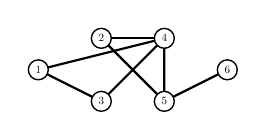
\begin{tikzpicture}[scale=0.4, every node/.style={scale=0.4}]
                            \Vertex[x=0, y=0]{1}
                            \Vertex[x=2, y=1]{2}
                            \Vertex[x=2, y=-1]{3}
                            \Vertex[x=4, y=1]{4}
                            \Vertex[x=4, y=-1]{5}
                            \Vertex[x=6, y=0]{6}

                            \Edge(3)(1)
                            \Edge(4)(1)
                            \Edge(4)(2)
                            \Edge(4)(3)
                            \Edge(5)(2)
                            \Edge(5)(4)
                            \Edge(6)(5)
                        \end{tikzpicture} and $H$:
                        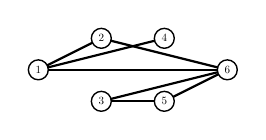
\begin{tikzpicture}[scale=0.4, every node/.style={scale=0.4}]
                            \Vertex[x=0, y=0]{1}
                            \Vertex[x=2, y=1]{2}
                            \Vertex[x=2, y=-1]{3}
                            \Vertex[x=4, y=1]{4}
                            \Vertex[x=4, y=-1]{5}
                            \Vertex[x=6, y=0]{6}

                            \Edge(2)(1)
                            \Edge(4)(1)
                            \Edge(5)(3)
                            \Edge(6)(1)
                            \Edge(6)(2)
                            \Edge(6)(3)
                            \Edge(6)(5)
                        \end{tikzpicture}. Now, we can (for example) re-label
                        our drawing of $H$ so that the edges joining label
                        pairs match $G$ as follows $H$:
                        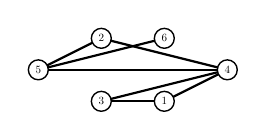
\begin{tikzpicture}[scale=0.4, every node/.style={scale=0.4}]
                            \Vertex[x=0, y=0]{5}
                            \Vertex[x=2, y=1]{2}
                            \Vertex[x=2, y=-1]{3}
                            \Vertex[x=4, y=1]{6}
                            \Vertex[x=4, y=-1]{1}
                            \Vertex[x=6, y=0]{4}

                            \Edge(3)(1)
                            \Edge(4)(1)
                            \Edge(4)(2)
                            \Edge(4)(3)
                            \Edge(5)(2)
                            \Edge(5)(4)
                            \Edge(6)(5)
                        \end{tikzpicture}.
                \end{enumerate}
            \end{enumerate}
        \pagebreak
        \item
            \begin{enumerate}
                \item
                    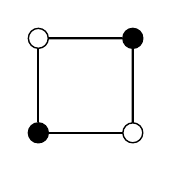
\begin{tikzpicture}[scale=0.6, every node/.style={scale=0.6}]
                        \SetVertexNoLabel
                        \GraphInit[vstyle=Classic]
                        \Vertex[x=0, y=0]{1}
                        \Vertex[x=2, y=2]{3}

                        \SetVertexSimple[LineColor = black, FillColor = white]
                        \Vertex[x=2, y=0]{2}
                        \Vertex[x=0, y=2]{4}

                        \Edge(1)(4)
                        \Edge(1)(2)
                        \Edge(3)(4)
                        \Edge(3)(2)
                    \end{tikzpicture}
                \item
                    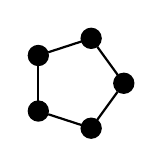
\begin{tikzpicture}[scale=0.6, every node/.style={scale=0.6}]
                        \SetVertexNoLabel
                        \GraphInit[vstyle=Classic]
                        \Vertices{circle}{1,2,3,4,5}
                        \Edges(1,2,3,4,5,1)
                    \end{tikzpicture}
                \item If a graph has no triangles, $m \leq 2n - 4$ where $m$ is
                    the number of edges and $n$ the number of vertices in the
                    graph. By inspection, $J$ has no triangles, 8 vertices and
                    12 edges. Hence $n = 8$ and $m = 12$ and $m \leq 2n-4$ is
                    true. It is therefore possible (but not certain) that $J$
                    is planar. Let's draw $J$ with a different vertex layout to
                    demonstrate its planarity.

                    $J$: 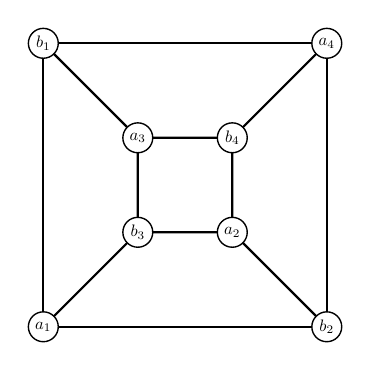
\begin{tikzpicture}[scale=0.6, every node/.style={scale=0.6}]
                        \Vertex[L=$a_1$, x=0, y=0]{a1}
                        \Vertex[L=$b_2$, x=6, y=0]{b2}
                        \Vertex[L=$b_3$, x=2, y=2]{b3}
                        \Vertex[L=$a_2$, x=4, y=2]{a2}
                        \Vertex[L=$a_3$, x=2, y=4]{a3}
                        \Vertex[L=$b_4$, x=4, y=4]{b4}
                        \Vertex[L=$b_1$, x=0, y=6]{b1}
                        \Vertex[L=$a_4$, x=6, y=6]{a4}

                        \Edge(a1)(b1)
                        \Edge(a1)(b2)
                        \Edge(a1)(b3)
                        \Edge(a2)(b2)
                        \Edge(a2)(b3)
                        \Edge(a2)(b4)
                        \Edge(a3)(b1)
                        \Edge(a3)(b3)
                        \Edge(a3)(b4)
                        \Edge(a4)(b4)
                        \Edge(a4)(b2)
                        \Edge(a4)(b1)

                    \end{tikzpicture}

                    $K$ is easier to classify, since $m = 20$ and $n = 10$ so
                    observing that $K$ has no triangles and testing against the
                    condition of planarity mentioned above
                    \begin{align*}
                        m &\leq 2n - 4 \\
                        20 &\leq 2 \cdot 10 - 4 \\
                           &\leq 20 - 4 \\
                        20 &\leq 16 \\
                    \end{align*}
                    which is clearly false and as such $K$ is non-planar.
            \end{enumerate}
        \item Prim's algorithm starting with $T = (\{f\}, \{\})$, edges are
            added in  the following order $\{f, c\}, \{c, e\}, \{e, d\}, \{d,
            a\}, \{c, b\}$ giving the minimum tree

            $T$: 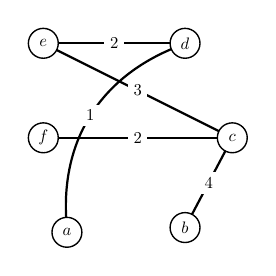
\begin{tikzpicture}[scale=0.6, every node/.style={scale=0.6}]
                \Vertex[L=$a$, x=0.5, y=0]{a}
                \Vertex[L=$f$, x=0, y=2]{f}
                \Vertex[L=$e$, x=0, y=4]{e}
                \Vertex[L=$d$, x=3, y=4]{d}
                \Vertex[L=$c$, x=4, y=2]{c}
                \Vertex[L=$b$, x=3, y=0.1]{b}

                \Edge[label=2](f)(c)
                \Edge[label=3](c)(e)
                \Edge[label=2](e)(d)
                \Edge[label=1, style={bend right=35}](d)(a)
                \Edge[label=4](c)(b)
            \end{tikzpicture} with total weight 12.
        \item
            \begin{enumerate}
                \item Dropping and adding vertices in the following sequence
                    $$
                    \begin{array}{c|c}
                        \text{Drop} & \text{Add} \\
                        \hline
                        1 & 10 \\
                        2 & 6 \\
                        3 & 10 \\
                        4 & 5 \\
                        7 & 5 \\
                        5 & 10 \\
                        8 & 6 \\
                        9 & 6 \\
                        6 & 10 \\
                    \end{array}
                    $$
                    gives the Pr{\"u}fer sequence $[10, 6, 10, 5, 5, 10, 6, 6, 10]$.
                \item The Pr{\"u}fer sequence $[3,3,4,3,3,5,4]$ gives the tree

                        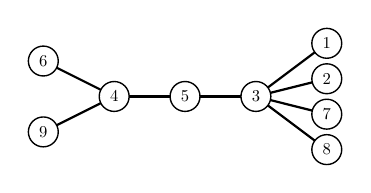
\begin{tikzpicture}[scale=0.9, every node/.style={scale=0.6}]

                            \Vertex[x=0, y=0]{9}
                            \Vertex[x=0, y=1]{6}
                            \Vertex[x=1, y=0.5]{4}
                            \Vertex[x=2, y=0.5]{5}
                            \Vertex[x=3, y=0.5]{3}
                            \Vertex[x=4, y=1.25]{1}
                            \Vertex[x=4, y=0.75]{2}
                            \Vertex[x=4, y=0.25]{7}
                            \Vertex[x=4, y=-0.25]{8}

                            \Edge(9)(4)
                            \Edge(6)(4)
                            \Edge(4)(5)
                            \Edge(5)(3)
                            \Edge(3)(8)
                            \Edge(3)(7)
                            \Edge(3)(2)
                            \Edge(3)(1)
                        \end{tikzpicture}.

                    I also implemented an algorithm to draw trees from
                    Pr{\"u}fer sequences using a computer
                    https://bmcorser.github.io/2017/02/04/prufer.html\#fun
                \item $n^{n-2}$ where $n = 8$ is $8^6 = 262144$.
                \item Labelling the tree presented with letters $a$ through
                    $h$, we can draw it as
                    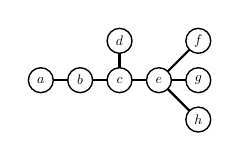
\begin{tikzpicture}[scale=0.5, every node/.style={scale=0.5}]
                        \Vertex[L=$a$, x=0, y=0]{a}
                        \Vertex[L=$b$, x=1, y=0]{b}
                        \Vertex[L=$c$, x=2, y=0]{c}
                        \Vertex[L=$d$, x=2, y=1]{d}
                        \Vertex[L=$e$, x=3, y=0]{e}
                        \Vertex[L=$f$, x=4, y=1]{f}
                        \Vertex[L=$g$, x=4, y=0]{g}
                        \Vertex[L=$h$, x=4, y=-1]{h}

                        \Edge(a)(b)
                        \Edge(b)(c)
                        \Edge(c)(d)
                        \Edge(c)(e)
                        \Edge(e)(f)
                        \Edge(e)(g)
                        \Edge(e)(h)
                    \end{tikzpicture}. Now, the number of ways of choosing a
                    label for vertex $c$ is 8, the number of ways of choosing
                    labels for those vertices adjacent to $c$ ($b$, $d$ and
                    $e$) is $\binom{7}{3}$. The number of ways of choosing
                    labels for $a$, $f$, $g$ and $h$ are 4, 3, 2 and 1. So the
                    number of labelling schemes is $8 \cdot \binom{7}{3} \cdot
                    4 \cdot 3 \cdot 2 \cdot 1 = 6720$
            \end{enumerate}
    \end{enumerate}
\end{document}

